\documentclass[]{beamer}

\usepackage[brazil]{babel}
\usepackage[utf8]{inputenc}
\usepackage{graphicx}
\usepackage{tikz}

\title{{\tt \href{https://github.com/ajholanda/nixus/wiki}{nixus}} -
  Comparação de deslocamentos de imagens RF} \author{Adriano
  J. Holanda$^0$, Antônio Adilton Carneiro$^1$}
\institute{$^0$Departamento de Computação e
  Matemática\\$^1$Departamento de Física\\FFCLRP--USP} \date{7 de
  dezembro de 2012}

\begin{document}

\frame{\maketitle}

\frame{\frametitle{Trilha}\tableofcontents}

\section{Introdução}

\frame{\author{}\date{}\institute{}\title{Introdução}\maketitle}

\begin{frame}{Dados de RF}
  
  Sonix RP coleta dados de Rádio Frequência (RF) digital antes de
  qualquer processamento, tais como. filtro, detecção de envelope e
  compressão.

  \begin{figure}
    \centering
    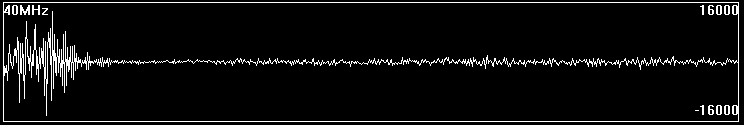
\includegraphics[scale=.4]{img/RFspectrum.png}
  \end{figure}

\end{frame}

\begin{frame}{RF: dados}

\def\rfdatascale{0.6}
\colorlet{h0}{red}
\colorlet{h1}{blue}
\colorlet{h2}{green!60!black!90}
\colorlet{fileheader}{gray!40!black!70}
  \begin{tikzpicture}
    [sample/.style={anchor=east,font=\tiny,minimum width=\rfdatascale cm,minimum height=.5cm,draw},
      hmax/.style={sample,anchor=west,minimum width=1cm}]
    
    \node[font=\tiny,draw] at (-3.75cm,3) {\color{fileheader}76-byte file header};
    
    \def\slabel{{\ifnum\x=-1{4-byte frame header} %
        \else\ifnum\x=9{$\ldots$} %
        \else\x\fi\fi}} %
    \foreach \x in {-1,0,1,...,8,9} {
      \node[sample] (p3\x) at (\rfdatascale*\x cm,3) {\color{h0}{\slabel}};
      \node[sample] (p2\x) at (\rfdatascale*\x cm,2) {\color{h1}{\slabel}};
      \node[sample] (p1\x) at (\rfdatascale*\x cm,1) {\color{h2}{\slabel}};
    }
    \node[hmax] [right of=p39,xshift=-.2cm] {\color{h0}$h-1$};
    \node[hmax] [right of=p29,xshift=-.2cm] {\color{h1}$h-1$};
    \node[hmax] [right of=p19,xshift=-.2cm] {\color{h2}$h-1$};
    
    \end{tikzpicture}


  

\end{frame}

\section{Objetivo}

\begin{frame}{Objetivo}
  Desenvolvimento de um conjunto de programas para o estudo de
  elastografia em imagens RF (rádio-frequência) obtidas a partir de
  equipamento de ultrassom específico para pesquisa.
\end{frame}

\section{Metodologia}

\begin{frame}{Passos}

  \begin{enumerate}
  \item Leitor de RF;
  \item Medida de similaridade;
  \item Medida de deslocamento das regiões deformadas;
  \item Contrução do gráfico de deslocamentos.
  \end{enumerate}
  
\end{frame}

\begin{frame}{Medidas de similaridade}
\begin{itemize}
  \item {\color<2>{gray}{B-Spline}};
  \item {\only<2>{\bf}Correlação cruzada normalizada};
  \item {\color<2>{gray}Grafos};
   \item {\color<2>{gray}Soma das diferenças absolutas (\scriptsize\em
       SAD-sum of absolute differences)};
   \item {\color<2>{gray}Soma do quadrado das diferenças (\scriptsize\em
       SSD-sum of squared differences)}.


\end{itemize}
\end{frame}

\begin{frame}{Por quê Correlação Cruzada?}
  \begin{itemize}\footnotesize
    \item Operação aritméticas simples;
    \item Identificação da aleatoriedade de um
      sequência $(k+1)$-distribuída usando correlação serial~\cite{taocp2}:
      \begin{equation}
        \lim_{n\to\infty}\frac{\frac{1}{n}\sum x_ix_{i+k}-
          (\frac{1}{n}\sum x_i)(\frac{1}{n}\sum x_{i+k})}
        {\sqrt{(\frac{1}{n}\sum x_i^2-(\frac{1}{n}\sum x_i)^2)
          (\frac{1}{n}\sum x_{i+k}^2-(\frac{1}{n}\sum x_{i+k})^2)}}=0
      \end{equation}
      \hfil $0\geq i<n \wedge x \in (0..1]$
      
  \end{itemize}
\end{frame}

\begin{frame}{Correlação cruzada}{Fórmula original}

Ineficiente, $O(n^2)$: 2 passadas pelo conjunto de dados.

\begin{enumerate}
  \item Cálculo da média
  \item Cálculo da Correlação
\end{enumerate}

\begin{equation}
  \overline{x} = \frac{\sum{x_i}}{n}
\end{equation}

\begin{equation}
  r_{xy}= 
  \frac{
    \sum
    (x_i-\overline{x})(y_i- \overline{y})
  }{
    \sqrt{\sum (x_i-\overline{x})^2
      \sum (y_i-\overline{y})^2},
  }  
\label{a}
\end{equation}
{\footnotesize $1\leq i\leq n$}
\end{frame}

\begin{frame}{Correlação cruzada}{Fórmula modificada}

$O(n)$, somente uma passada pelo conjunto de dados.

\begin{equation}
  r_{xy} = 
    \frac{
      n\sum x_iy_i-\sum x_i\sum y_i
    }
        {
          \sqrt{n\sum x_i^2-(\sum x_i)^2}
          \sqrt{n\sum y_i^2-(\sum y_i)^2}
        }
\end{equation}
{\footnotesize $1\leq i\leq n$}
\end{frame}

\begin{frame}{Otimização do cálculo de correlação cruzada}
  \begin{itemize}
  \item Dependendo do número de elementos na série $O(n)$, ainda é insatisfatório;
  \item Otimização usando recursos de hardware, principalmente o processador;
  \item Porém outros componentes podem ser otimizados, por exemplo,
    entrada/saída, números de threads de execução.
  \end{itemize}  
\end{frame}


\begin{frame}{Otimização: processador}

  \begin{block}{x86-64 (Intel/AMD)}
    \begin{itemize}
    \item Introdução de extensões para operações multimídia, através do
      SSE (Streaming SIMD\footnote{single instruction, multiple data} Extensions);
    \item Aumento da capacidade dos registradores (XMM) para $128$
      bits, com a implementação de operações compostas.
    \end{itemize}
  \end{block}

\begin{center}
  \begin{tikzpicture}[memslot/.style={minimum height=.5cm,minimum
      width=1cm,font=\tiny,draw}, xmm/.style={color=red}]
   

    \foreach \x in {0,1,2,3,4,5,6,7} {
      \ifnum\x<4{
      \node[memslot] (reg\x) at (\x cm,0) {16-bit};
    }\fi
      \node[memslot,xmm] (xmm\x) at (\x cm,-1cm) {16-bit};
    }
    \node [left of=reg0,xshift=-.5cm] {REG};
    \node[xmm] [left of=xmm0,xshift=-.5cm] {XMMx};
    

  \end{tikzpicture}
\end{center}

\end{frame}

\begin{frame}{SSE: Operações compostas}
  \def\x{111}
  \def\y{222}
  \def\w{444}
  \def\z{555}
  \begin{tikzpicture}[reg/.style={draw}]

\node (std) {Instrução padrão};

\only<1> {
    \node[font=\tt] (addc0) [below of=std] {add};
    \node[reg,blue] (xc) [right of=addc0] {$\x$};
    \node[anchor=south] (plusc0) [right of=xc,xshift=-.3cm] {$,$};
    \node[reg,red] (yc) [right of=plusc0,xshift=-.3cm] {$\y$};
    \node[font=\tt] (addc1) [below of=addc0] {add};
    \node[reg,brown] (wc) [right of=addc1] {$\w$};
    \node[anchor=south] (plusc1) [right of=wc,xshift=-.3cm] {$,$};
    \node[reg,cyan] (zc) [right of=plusc1,xshift=-.3cm] {$\z$};
}
   
\only<2>{
  \node [right of=std, xshift=1.5cm] {\small $\Rightarrow$ 2 ciclos};

  \node[reg,blue] (rxc) [below of=std] {$333$};
  \node[reg,red] (ryc) [below of=rxc] {$999$};
}


\node (sse) [below of=std, yshift=-2.5cm] {Instrução SSE: adição};

\only<1> {
    \node[font=\tt] (addsse) [below of=sse,yshift=-.5cm] {paddq};
    \node[reg,blue] (xsse) [right of=addsse,xshift=.5cm] {$\x$};
    \node[reg,blue] (ysse) [right of=xsse,xshift=-.15cm] {$\y$};
    \node[reg,blue] (wsse) [right of=ysse,xshift=-.15cm] {$\w$};
    \node[reg,blue] (zsse) [right of=wsse,xshift=-.15cm] {$\z$};
    \node[anchor=south] (plussse) [right of=zsse,xshift=-.3cm] {$,$};
    \node[reg,blue] (sxsse) [right of=plussse] {$\x$};
    \node[reg,blue] (sysse) [right of=sxsse,xshift=-.15cm] {$\y$};
    \node[reg,blue] (swsse) [right of=sysse,xshift=-.15cm] {$\w$};
    \node[reg,blue] (szsse) [right of=swsse,xshift=-.15cm] {$\z$};
}

\only<2>{
  \node [right of=sse, xshift=1.5cm] {\small $\Rightarrow$ 1 ciclo};

  \node[reg,blue] (rxsse) [below of=sse] {$333$};
  \node[reg,blue,text=gray] (rysse) [right of=rxsse,xshift=-.15cm] {$\y$};
  \node[reg,blue] (rwsse) [right of=rysse,xshift=-.15cm] {$999$};
  \node[reg,blue,text=gray] (rzsse) [right of=rwsse,xshift=-.15cm] {$\z$};
}

  \end{tikzpicture}
    
\end{frame}

\begin{frame}{{\em Benchmark} \tt xcorr}
  \small
  $9\times 10^7\text{pontos} \Rightarrow  \delta_\text{\sc SSE}/\delta_\text{\sc
    C} = 0.5558$\hfill {\scriptsize $\delta$ - número de ciclos}
\begin{center}
    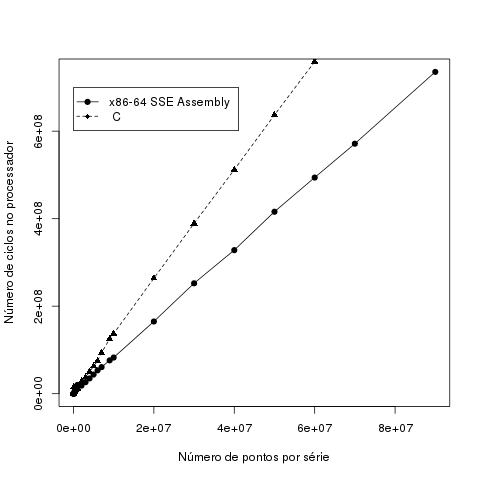
\includegraphics[scale=.425]{xcorr-bench.png}
  \end{center}
\end{frame}


\section{Discussões}

\begin{frame}{Outros pontos de otimização}

  \begin{itemize}
  \item Entrada/saída não bloqueante;
  \item Múltiplas {\em threads} de execução para redução do custo de
    criação do processo;
  \item Evitar uso de cache armazenando os dados no registrador;
  \item Intel I7 possui extensão AVX\footnote{\em Advanced Vector
      Extensions} com intruções de 256 bits.
  \end{itemize}
  
\end{frame}

\section{Cronograma}

\begin{frame}{Cronograma}
\begin{center}
{\Large\only<1>{Realizações em 2012}
\only<2>{Estimativa para 2013}}
\end{center}
\begin{center}
\begin{tabular}{|c|c|}\hline
  \color<2>{gray} 1$^o$sem2012 & \color<2>{gray} Estudo RF, Revisão da Literatura e Especificação \\\hline
  \color<2>{gray} 2$^o$sem2012 & \color<2>{gray} Estrutura de dados RF
  e Correlação Cruzada \\\hline
   \color<1>{gray}     {\bf 1$^o$sem2013} & \color<1>{gray} varredura procurando deslocamentos \\\hline
   \color<1>{gray} {\bf 2$^o$sem2013 } & \color<1>{gray} interface de programação \\\hline
\end{tabular}
\end{center}
\end{frame}


\begin{frame}{Referências}
\begin{thebibliography}{4}

\bibitem{taocp2}[Knuth2, 1997]
The Art of Computer Programming: Seminumerical Algorithms
\newblock Donald E. Knuth
\newblock 3rd edition, vol. 2, 1997
\newblock Addison-Wesley Professional

\bibitem{sonixrpman}[SonixRP, 2006]
  \href{http://www.ultrasonix.com/webfm_send/634}{SonixRP Service
    Manual}.
  \newblock Ultrasonix Medical Corporation.
\end{thebibliography}
\end{frame}

\end{document}
